% file: 2-11-heapsort/heap-subtrees.tex
% containing 13 nodes

\documentclass[tikz]{standalone}
\usepackage{tikz-qtree}
\usetikzlibrary{backgrounds, fit, shapes}

\begin{document}
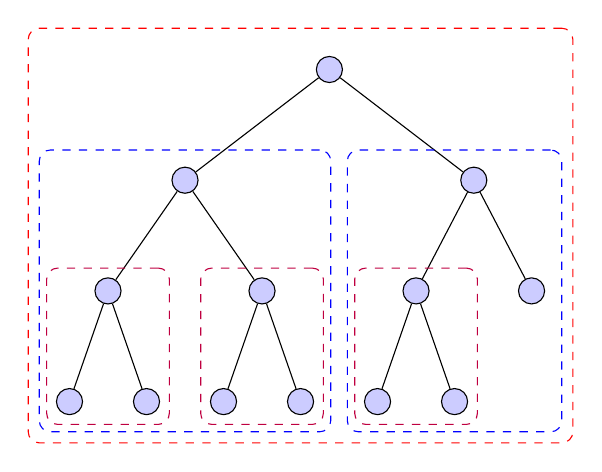
\begin{tikzpicture} [level distance = 40pt, sibling distance = 18pt,
  edge from parent/.style= { % added code
      draw, edge from parent path = {(\tikzparentnode) -- (\tikzchildnode)}},
    bg/.style = {draw, dashed, rounded corners, inner sep = #1}]
  \tikzset{every tree node/.style = 
    {align = center, circle, draw, fill = blue!20, font = \Large}}
    \Tree [.\node (t) {};
	     [.\node (l) {};
	       [.\node (ll) {}; 
		\node (lll) {};
		\node (llr) {};
	       ]
	       [.\node (lr) {};
	        \node (lrl) {};
		\node (lrr) {};
	       ]
            ]
	    [.\node (r') {};	% r may be reserved for ``root'' by tikz-qtree
	      [.\node (rl) {};
	       \node (rll) {};
	       \node (rlr) {};	
	      ]
	      \node (rr) {};
	   ] 
        ]
  
  \node () [bg = 10pt, red, fit = (t) (lll) (rr)] {};   

  \node () [bg = 6pt, blue, fit = (l) (lll) (lrr)] {};   
  \node () [bg = 6pt, blue, fit = (r') (rll) (rr)] {}; 

  \node () [bg, purple, fit = (ll) (lll) (llr)] {};   
  \node () [bg, purple, fit = (lr) (lrl) (lrr)] {}; 
  \node () [bg, purple, fit = (rl) (rll) (rlr)] {}; 
\end{tikzpicture}
\end{document}
